\documentclass[border=10pt]{standalone}
\usepackage[svgnames]{xcolor}
\usepackage{amsmath}
\usepackage{pgfplots}
\pgfplotsset{compat=newest}
\usepackage[sfdefault]{FiraSans}
\usepackage{FiraMono}
\renewcommand*\familydefault{\sfdefault}
\begin{document}
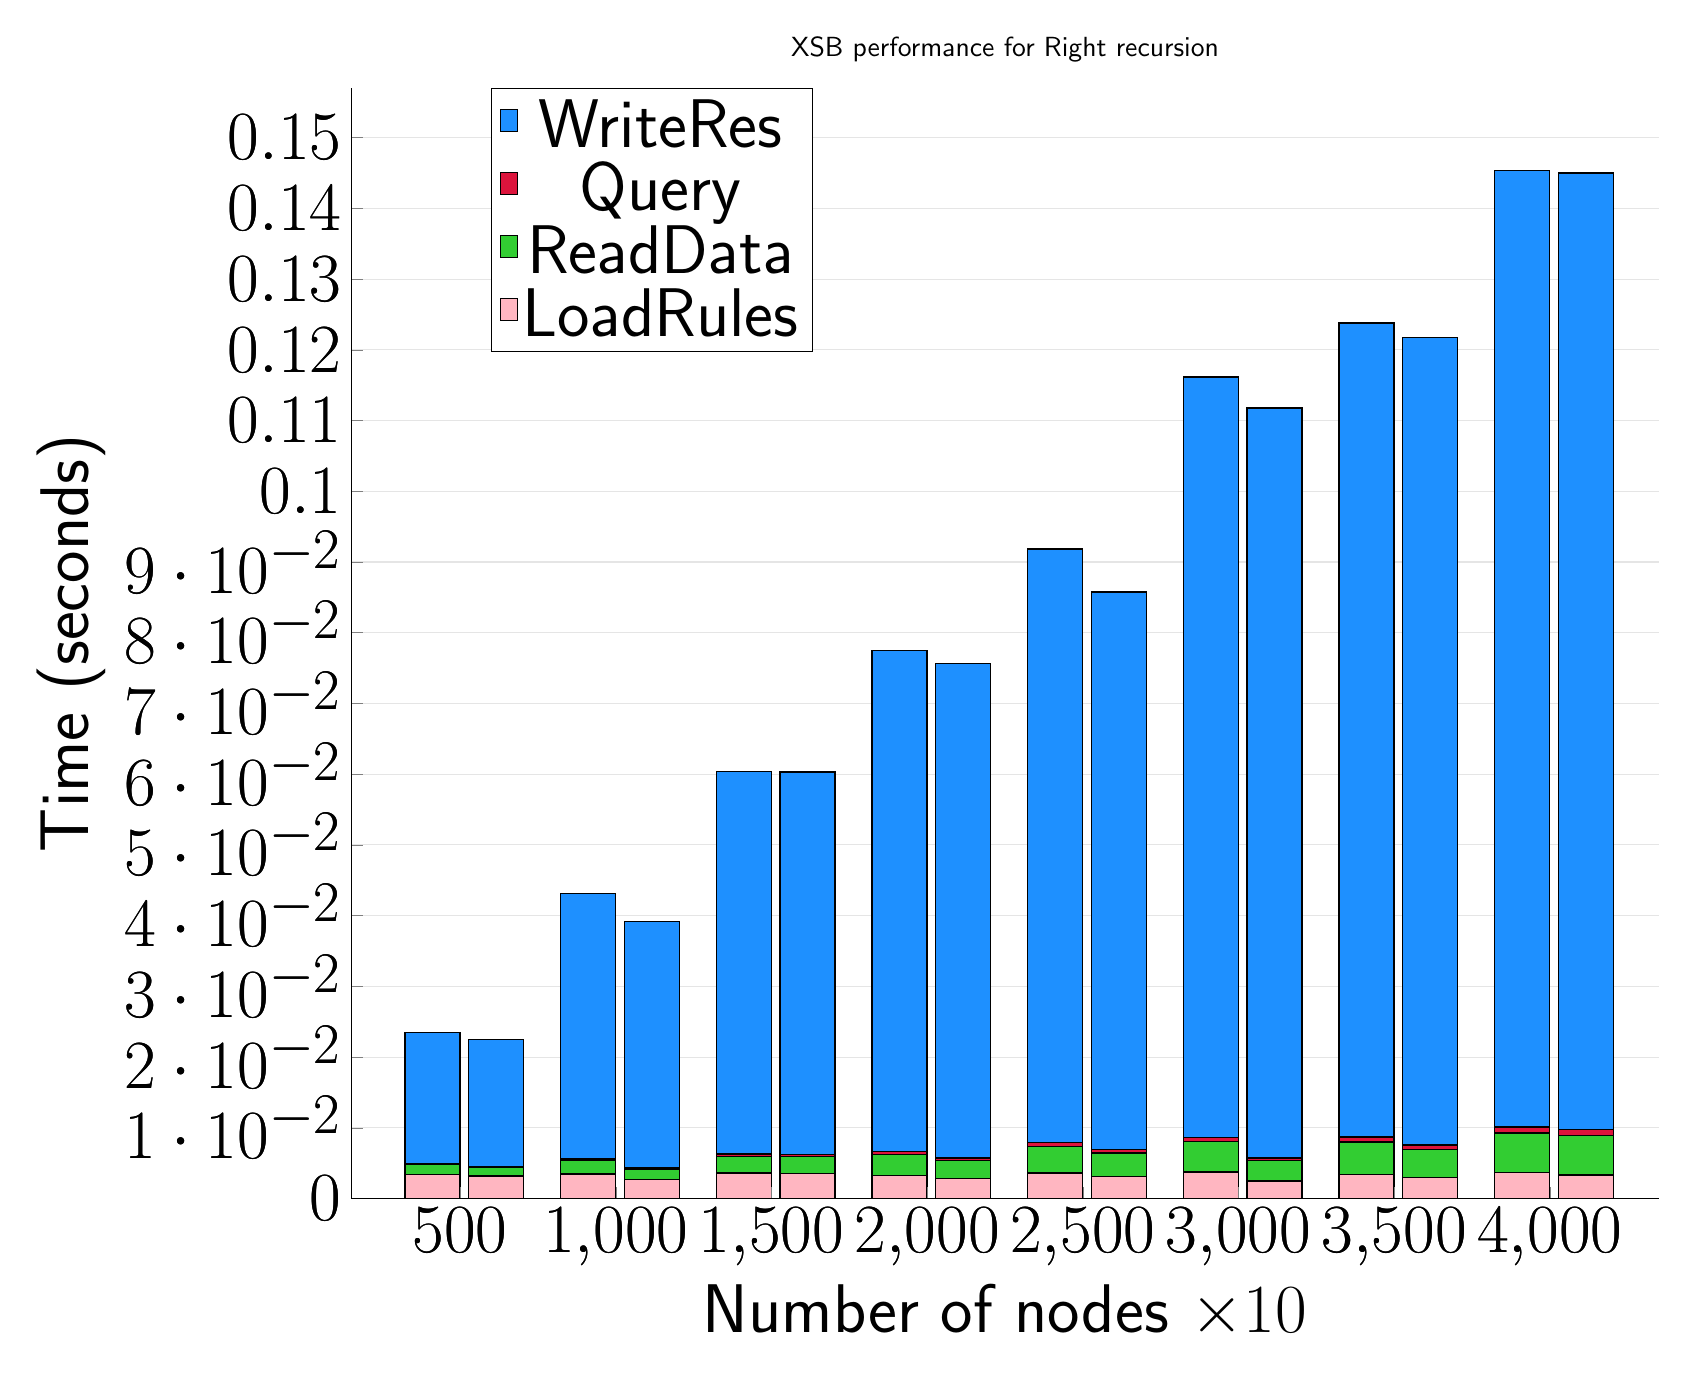
\begin{tikzpicture}
\begin{axis}[
   ybar stacked,
   title={XSB performance for Right recursion},
   bar shift=-10pt,
   width=1.5\textwidth,
   bar width=0.7cm,
   ymajorgrids, tick align=inside,
   major grid style={draw=gray!20},
   xtick=data,
   ymin=0, ymax=0.1570375951131183,
   axis x line*=bottom,
   axis y line*=left,
   enlarge x limits=0.1,
   legend style={
       at={(0.23, 1)},
       anchor=north,
       legend columns=1,
       font=\Huge,
   },
   ylabel={Time (seconds)},
   xlabel={Number of nodes $\times 10$},
   label style={font=\Huge},
   tick label style={font=\Huge},
]
\addlegendimage{fill=DodgerBlue, draw=black, line width=0.2pt}
\addlegendentry{WriteRes}
\addlegendimage{fill=Crimson, draw=black, line width=0.2pt}
\addlegendentry{Query}
\addlegendimage{fill=LimeGreen, draw=black, line width=0.2pt}
\addlegendentry{ReadData}
\addlegendimage{fill=LightPink, draw=black, line width=0.2pt}
\addlegendentry{LoadRules}
\addplot +[fill=LightPink, draw=black, line width=0.5pt] coordinates {
    (500, 0.00343171755472819)
    (1000, 0.00345826148986816)
    (1500, 0.0036009947458902993)
    (2000, 0.003266096115112307)
    (2500, 0.0036086241404215506)
    (3000, 0.003741741180419923)
    (3500, 0.003417015075683597)
    (4000, 0.003703991572062177)
};
\addplot +[fill=LimeGreen, draw=black, line width=0.5pt] coordinates {
    (500, 0.0013582706451415998)
    (1000, 0.0019310315450032569)
    (1500, 0.0023883183797200496)
    (2000, 0.0030055840810139967)
    (2500, 0.0037494500478108734)
    (3000, 0.00434263547261556)
    (3500, 0.00456690788269043)
    (4000, 0.005587339401245117)
};
\addplot +[fill=Crimson, draw=black, line width=0.5pt] coordinates {
    (500, 0.00012143452962239599)
    (1000, 0.0001983642578125)
    (1500, 0.0002926985422770183)
    (2000, 0.000406980514526367)
    (2500, 0.0005566279093424477)
    (3000, 0.0005699793497721357)
    (3500, 0.000709056854248047)
    (4000, 0.0008216698964436846)
};
\addplot +[fill=DodgerBlue, draw=black, line width=0.5pt] coordinates {
    (500, 0.01860721906026204)
    (1000, 0.03752851486206053)
    (1500, 0.054097731908162416)
    (2000, 0.07081802686055504)
    (2500, 0.08395147323608398)
    (3000, 0.10751732190450053)
    (3500, 0.11512136459350562)
    (4000, 0.13527965545654297)
};
\end{axis}
\begin{axis}[
   ybar stacked,
   bar shift=13pt,
   width=1.5\textwidth,
   bar width=0.7cm,
   ymajorgrids, tick align=inside,
   major grid style={draw=none},
   xtick=data,
   ymin=0, ymax=0.1570375951131183,
   axis x line*=none,
   axis y line*=none,
   enlarge x limits=0.1,
   label style={font=\Huge},
   tick label style={font=\Huge},
]
\addplot +[fill=LightPink, draw=black, line width=0.5pt] coordinates {
    (500, 0.003194666666666667)
    (1000, 0.0027096666666666697)
    (1500, 0.0035733333333333333)
    (2000, 0.002818666666666667)
    (2500, 0.003150666666666666)
    (3000, 0.002485333333333332)
    (3500, 0.002979666666666667)
    (4000, 0.0033323333333333334)
};
\addplot +[fill=LimeGreen, draw=black, line width=0.5pt] coordinates {
    (500, 0.0012673333333333332)
    (1000, 0.0014966666666666668)
    (1500, 0.0023883333333333335)
    (2000, 0.0025663333333333367)
    (2500, 0.0033176666666666667)
    (3000, 0.0028573333333333333)
    (3500, 0.003968666666666666)
    (4000, 0.005575)
};
\addplot +[fill=Crimson, draw=black, line width=0.5pt] coordinates {
    (500, 0.0001140000000000006)
    (1000, 0.00015299999999999567)
    (1500, 0.00029266666666666563)
    (2000, 0.000356666666666665)
    (2500, 0.000480000000000001)
    (3000, 0.0003720000000000043)
    (3500, 0.000628000000000001)
    (4000, 0.0008206666666666678)
};
\addplot +[fill=DodgerBlue, draw=black, line width=0.5pt] coordinates {
    (500, 0.017928)
    (1000, 0.034779666666666674)
    (1500, 0.05407766666666667)
    (2000, 0.069883)
    (2500, 0.078834)
    (3000, 0.10607233333333332)
    (3500, 0.11414466666666667)
    (4000, 0.13527466666666665)
};
\end{axis}
\end{tikzpicture}

\end{document}
